\documentclass[conference]{IEEEtran}
\IEEEoverridecommandlockouts
% The preceding line is only needed to identify funding in the first footnote. If that is unneeded, please comment it out.
\usepackage{cite}
\usepackage{amsmath,amssymb,amsfonts}
\usepackage{algorithmic}
\usepackage{graphicx}
\usepackage{textcomp}
\usepackage{xcolor}
\usepackage{listings}
\def\BibTeX{{\rm B\kern-.05em{\sc i\kern-.025em b}\kern-.08em
    T\kern-.1667em\lower.7ex\hbox{E}\kern-.125emX}}


\lstset{captionpos=b, numberbychapter=false,caption=\lstname,frame=none, numbers=left, stepnumber=1, numbersep=2pt, xleftmargin=2pt, framexleftmargin=2pt, numberstyle=\tiny, tabsize=3, columns=fixed, basicstyle={\fontfamily{pcr}\selectfont\footnotesize}, keywordstyle=\bfseries, commentstyle={\color[gray]{0.33}\itshape}, stringstyle=\color[gray]{0.25}, breaklines, breakatwhitespace, breakautoindent}
\lstloadlanguages{[ANSI]C, C++, [gnu]make, gnuplot, Matlab}

\begin{document}

\bibliographystyle{IEEEtran}

\title{Microservices: Use of REST and gRPC over SOAP}

\author{\IEEEauthorblockN{Marcel Gredler}
\IEEEauthorblockA{\textit{Computer Science} \\
\textit{FH Technikum Wien}\\
Vienna, Austria \\
se19m025@technikum-wien.at}
\and
\IEEEauthorblockN{Florencia Cavallin}
\IEEEauthorblockA{\textit{Computer Science} \\
\textit{FH Technikum Wien}\\
Vienna, Austria \\
se19m501@technikum-wien.at}
}

\maketitle

\begin{abstract}

Since the induction of Web Services into modern applications, their usage has grown. Together with them the general public was first introduced to the use of protocols like the Simple Object Access Protocol (SOAP) and Representational State Transfer (REST).

In more recent years a new trend started emerging in the development of applications, in which the application is split into a set of small services that use a communication protocol to interact with another. This trend is known as the Microservice Architecture and it favors the use of REST, a Message Bus or other stateless communication protocols over SOAP.

This paper gives an overview of the Microservice Architecture, explains why the use of REST is favored over SOAP and how the new gRPC Remote Procedure Calls (gRPC) framework may support them.

\end{abstract}

\begin{IEEEkeywords}
services, rest, grpc, microservices
\end{IEEEkeywords}

\section{Introduction}

Nowadays their exist many different paradigms and architectures that can be used to create applications. One of these architectural styles is the Service Oriented Architecture (SOA), in which the functionality is split between multiple services that may be run locally or be distributed around the network.

One methodology that heavily uses this paradigm and that is in widespread use, are web services \cite{halili2018web}. Within the use of web services applications can benefit by reusing the functionality of already existing other services. Because of this it is possible to reduce the need of rewriting existing functionality into every application. Another benefit is the possibility of sharing information between all such web services. To achieve all these benefits, web services traditionally employ the Simple Object Access Protocol (SOAP) or Representation State Transfer (REST) protocols \cite{halili2018web}.

Another methodology that became widespread between 2010 and 2020 are microservices. Where web services focused on offering a full service to another application or user, microservices are built around the offering and using of capabilities \cite{karmel2016nist}. Each capability is thereby built and offered as its own service and all communication is performed through an Application Programming Interface (API). A set of microservices can therefore build an application or be used to provide capabilities to other applications.

Since microservices are using lightweight protocols \cite{karmel2016nist} to communicate with each other, a protocol like REST is preferred over SOAP. One of the biggest advantages of REST over SOAP is the smaller payload, as SOAP may require the services to exchange ten times more bytes between each other in comparison to REST \cite{halili2018web}. Since microservices are built around capabilities and interaction between each other, a smaller payload allows for better use of the available bandwidth.
Additionally, changing the provisioning in SOAP may require changes on the clients, whereas REST does not \cite{halili2018web}. This is another important advantage, as microservices are generally designed to be independently deployable \cite{karmel2016nist}, which would be broken, if the deployment of one service requires the deployment of another.

With the from 2015 slowly emerging HTTP/2 standard \cite{rfc7540} another communication framework has been developed: gRPC Remote Procedure Calls (gRPC) \cite{GRPCAuthors2020}. While previously microservices only used REST, this new framework allows for the use of both gRPC and REST to interact with another. The gRPC framework thereby offers the ability to build so called gRPC REST Gateways \cite{grpcrest}. These gateways are proxies for that expose the gRPC capability through REST. This means that other services are able to use them with gRPC - if they so support this too - or use the REST API. The latter is especially useful in networks where HTTP/2 traffic is not yet fully supported, if for example used loadbalancer only support HTTP/1.1 yet.

This paper gives an introduction of the mentioned protocols SOAP, REST and gRPC. Furthermore it explains what microservices are and how the compare to a classical service oriented architecture. Lastly, the document explains the benefit of using HTTP/2 and gRPC in conjunction with a microservice architecture.

To achieve this goal, the paper is structured as follows: Sections \ref{sec:soap} to \ref{sec:grpc} cover the explanation about SOAP, REST and gRCP respectively. Section \ref{sec:micros} is about microservices and their comparison to the service oriented architecture. This is followed by sections \ref{sec:comp} and \ref{sec:compgrpc} which contain the benefits of using gRPC and REST. Lastly, the document finished by providing a conclusion about the use of gRPC and REST in microservices.

\section{SOAP}
\label{sec:soap}

SOAP is an XML based and small overhead protocol used for data exchange in distributed and decentralized systems.
It was developed by Microsoft DevelopMentor, Userland Software, and IBM. The W3C organization has established the specification of SOAP. W3C was founded in 1994 and is supported by several companies worldwide. \cite{SOA-basic-overview-2002}

SOAP supports different styles of information exchange. It supports Remote Procedure Call(RPC) style, which allows request-response processing and message-oriented information exchange, which is useful if you like to exchange business documents or other documents where the sender may not respond immediately. \cite{SOA-basic-overview-2002}

The Service Web is powered by Web application servers that speak SOAP and deliver information marked up in XML. To invoke a Web Service, the application needs information about the service given by a Web Service Description Language (WSDL) document. The WSDL documents are indexed in searchable Universal Description Discovery and Integration business registers (UDDI) that tell where the Web Services are located. \cite{SOA-basic-overview-2002} Web services are a way to connect different systems and programs over the Internet, despite differences in a programming language or system implementation.

The SOAP protocol consists of three main items:

\begin{itemize}
  \item The SOAP envelope: defines an overall framework for expressing what is in a message, who should deal with it, and whether it is optional or mandatory.
  \item The SOAP encoding rules: define a serialization mechanism that can be used to exchange instances of application-defined datatypes.
  \item The SOAP RPC representation: defines a convention that can represent remote procedure calls and responses.
\end{itemize}


SOAP can be used in combination with other protocols; however, it is usually used with HTTP.

This protocol was designed to be a more simple and extensible protocol than the ones already existing. Therefore some features that are usually in traditional messaging systems and distributed object systems were excluded, for example, distributed garbage collection, Objects-by-reference, Activation.

\subsection{The SOAP Message Exchange Model}

SOAP are unilateral communications from a transmitter to a receiver, but a system utilizing SOAP messages can also be implemented with a request/response scheme.
SOAP implementations can be optimized to take advantage of the particularities of the network system it is running on.
Messages are routed along a message path which allows for processing at one or more intermediate nodes in addition to the ultimate destination.
A SOAP application receiving a SOAP message processes the message in the following way:

\begin{itemize}
  \item It identifies all parts of the SOAP message intended for that application.
  \item Verify that the application supports all mandatory parts identified.
  \item Process all parts accordingly.
  \item If the SOAP application is not the ultimate destination, remove all parts identified and forward it.
\end{itemize}

\subsection{Relation to XML}

All SOAP messages are encoded using XML. A SOAP message is an XML document that consists of a mandatory SOAP envelope, an optional SOAP header, and a mandatory SOAP body. 

Figure 1 shows a SOAP Message Structure representation for a better understanding. This XML document is referred to as a SOAP message for the rest of this specification. The Envelope is the top element of the XML document representing the message. The Header is a generic mechanism for adding features to a SOAP message in a decentralized manner without prior agreement between the communicating parties. \cite{SOA-W3C-2000}

SOAP defines a few attributes that can indicate who should deal with a feature and whether it is optional or mandatory. The Body is a container for mandatory information intended for the ultimate recipient of the message.\cite{SOA-W3C-2000}

\begin{figure}
	\centering
	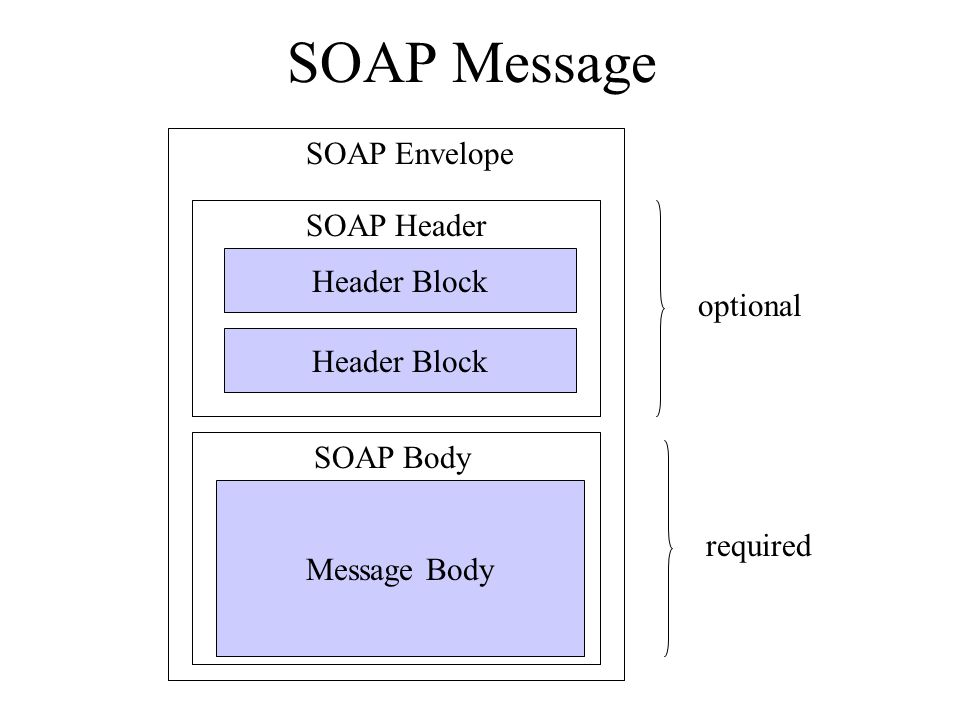
\includegraphics[width=0.8\linewidth]{soap_message.jpg}
	\caption{SOAP Message Structure Representation (Image downloaded from https://slideplayer.com/slide/3415118/ in January 2021)}
\end{figure}

\subsection{Advantages of SOAP}

The fact that it is based on a highly-structured format of XML can be considered a positive aspect because of its language simplicity and portability since no dependencies on the underlying platform are needed. Its Firewall friendliness can also help as the only requirement needed is to post data over HTTP. Open standards are used, which also brings interoperability and universal acceptance since its one of the most widely accepted message communication standards.

\subsection{Disadvantages of SOAP}

Too much reliance on HTTP can be a negative aspect, it is limited only to the request-response model, and HTTP's slow protocol can cause bad performance. It is stateless, making it difficult for transactional and business processing applications and serialization by value and by reference (impossible to refer or point to external data source).

\section{REST}
\label{sec:rest}

REST is an architectural style created and defined by Roy T. Fielding in his doctoral thesis. His objective was to use REST as a way to communicate the basic concepts underlying the Web. 

It is of great use to understand the definition of a resource, representation, and state. A resource can be anything. A resource may be a physical object or an abstract concept. As long as something is important enough to be referenced as a thing itself, it can be exposed as a resource. A resource is something that can be stored on a computer and represented as a stream of bits. \cite{Rest-WebServices-2009}

There are two types of state, the resource state (information about a resource) and the application state (information about the path the client has taken through the application).

REST provides a set of architectural constraints that, when applied as a whole, emphasizes scalability of component interactions, \cite{Rest-WebServices-2009} the generality of interfaces, independent deployment of components, and intermediary components to reduce interaction latency, enforce security, and encapsulate legacy systems.

\subsection{REST constraints}

\begin{itemize}
  \item Everything is a resource.
  \item Resource are identified through URIs.
  \item Uniform interface.
  \item Manipulation of resources through representations.
  \item Self-descriptive messages.
  \item Stateless interactions.
  \item Hypermedia as the engine of application state.
\end{itemize}

\subsection{Interfaces}

The most remarkable characteristic of REST is that it exposes the same interfaces to the client. 

The most known implementation of this protocol is with HTTP. It is a state transfer protocol other than a data transport protocol, but HTTP can also uniquely locate a resource and tell us how to operate it. This protocol demands that the requests and responses are performed with an HTTP operation: GET, POST, PUT and DELETE. 

Uniform interface becomes the Babel of interface definition. It helps to decouple between the client and the server and makes the client and the server evolve independently. As long as the interface remains unchanged, the client and the serve can interact normally.

\subsection{Scalability}

Stateless interactions constrain can also enhance the scalability of RESTful architecture. Stateless interactions constrain demands that each client's request should contain all application states necessary to understand that request. None of the state information is kept on the server, and none of it is implied by previous requests, reducing the cost of enlarging the system scale. 

\subsection{Reduce coupling}

The way to handle data format in REST helps reduce coupling between the client and the server. Allowing services to handle multiple data formats means that the client and the service can select appropriate data formats for different data types, such as images, text, and spreadsheets.

\subsection{Security}

The REST security model is straightforward and effective. Everything is abstracted into a resource in REST, and every resource is identified through its unique URI. REST uses the standard verbs of HTTP, and each verb has exact semantics. Setting different permissions for four operations of a resource can make up different security policies. These settings can all be completed on an HTTP firewall. The difficulty of implementing security policy is very low.

\subsection{Addressability}

With addressability, users can describe precisely the information that they want to receive from the service. In REST, URIs should be defined for every resource or resource representation, and they contain all information required to address it.

\subsection{Connectedness}

The server can navigate the links and forms given in the representation. During this process, links play an essential role in connecting resources. This way, service customers can make a path through the application by following the links.

\subsection{Performance}

The protocol is based on existing standards widely used in Web and requires no additional standards; it uses HTTP protocol in data exchange. It also recommends that the client or intermediaries cache responses that serve as cacheable to eliminate unnecessary interaction for better performance. This makes it competitive in terms of performance, being the only market with these characteristics.

\subsection{Data Types}

When a client request is made via a RESTful API, it transfers a representation of the resource's state to the receiver. This information, or representation, can be delivered in several formats—for example, JSON, HTML, XLT, Python, PHP, or plain text. 
JSON can be one of the most used because it is language-agnostic and readable by humans and machines.\cite{REST-red-hat}

All of these features make REST a strong and robust protocol for microservices implementation.

\section{HTTP/2}

The state of the web report of the HTTP archive \cite{httpArchive} suggests that between December 2010 and 2020, the amount of kilobytes (KB) required to load a web page increased by about 318 percent. In other words, in 2010 a page consisted of a median 487.9 KB, whereas in 2020 a web page consists of 2042.3 KB. Such an increase in size is a challenge for both the network we use and the protocols our communication is built upon.

HTTP/1.1 tries to solve the problem of increased page sizes by allowing request pipeline and through the use of multiple parallel open connections. While this was a viable approach for many years, an IETF working group published the newer HTTP/2 specification RFC 7540 \cite{rfc7540} in 2015, with an update regarding TLS 1.3 having been published in RFC 8740 \cite{rfc8740}. This new protocol version promises to solve the problems of HTTP/1.1 that prevent it from being more efficient.

Protocol version HTTP/2 moves away from sending text over the web and instead replaces it with binary data. RFC 7540 \cite{rfc7540} and the IETF HTTP working group \cite{httpwgHTTP2} explain this decision through the argument that binary data is more efficient to parse, as it less error prone and does not require to keep traffic of special characters in the data.

Furthermore HTTP/2 reworks the way semantic information is send through the web (see RFC 7540 \cite{rfc7540} for details) with the goal of allowing multiple requests to be sent through the same connection. Based on the documents \cite{rfc7540} \cite{httpwgHTTP2} this decisions has been to make the HTTP/2 protocol more in line with how TCP connections work. For traffic to flow through an TCP connection, a handshake has to be done first between the two participants. In HTTP/1.1 this meant that for each parallel request a newly opened connection had to go through this very handshake again, instead of being able to use the handshake from the first request, overall increasing the overhead a user had to perform to download the content of a page. HTTP/2 on the other hand only opens one TCP connection minimizing this overhead. Additionally, the header of the HTTP/2 protocol itself are compressed while being send through the network, further reducing the size of each message.

Lastly, HTTP/2 introduces a new feature called server push \cite{rfc7540}. With this feature it is possible for a server to push additional information to the clients, based on their previous requests, without having to wait for them to open a request for this data themselves. Though introducing the ability to send "false-positive" data (i.e. data that is not used by the user in the end), this new feature allows the server to provide the user with "future" information without delay (from user perspective), which helps in providing a better user experience.

\begin{table}[!htbp]
	\centering
	\caption{HTTP/1.1 VS HTTP/2}
	\label{http2comparison}
	\begin{tabular}{| p{0.4\linewidth} | p{0.4\linewidth}|}\hline
		HTTP/1.1 & HTTP/2 \\\hline
		text-based protocol & binary protocol \\\hline
		one request per TCP connection & multiple requests per TCP connection \\\hline
		no header compression & header compression \\\hline
		only client may request data & client may request data and server may push additional data \\\hline
	\end{tabular}
\end{table}

To further highlight these core differences between how HTTP/1.1 and HTTP/2 treat their traffic, table \ref{http2comparison} provides a comparison of the two versions, reiterating the information provided by this section in a compact format.

The claims of performance improvement by use of HTTP/2 instead of HTTP/1 can be validated empirically. Corbel, Stephan and Omnes perform in their paper "HTTP/1.1 pipelining vs HTTP2 in-the-clear: Performance comparison" \cite{7745823} such an empirical study. They compare the time to download web pages by using the same infrastructure and server, with only the protocol version differing in the data-sets. As a result of their study they were able to identify that HTTP/2 truly does perform better than HTTP/1 for downloading content.

\section{gRPC}
\label{sec:grpc}

The gRPC Remote Procedure Calls (gRPC) framework \cite{GRPCAuthors2020} is a technology initially developed by Google and since having been become an open source framework maintained by the Cloud Native Computing Foundation (CNCF). It is a remote procedure call (RPC) framework that has been developed in modern times (beginning with 2015) and is backed by the HTTP/2 protocol. It has been created with the idea of a general purpose RPC infrastructure and microservice architectures in mind. This means that the created RPC framework was required to be language agnostic and allow for the fast and responsive intercommunication between a multitude of service instances.

Above requirements to the RPC protocol are reflected by the following principles of the gRPC design specification \cite{grpcmotiviation}:

\begin{itemize}
	\item \textbf{Services not objects}: gRPC allows for the communication with services and is not an object oriented.
	\item \textbf{Messages not References}: Client and server exchange messages between them and do not have references to objects.
	\item \textbf{Interoperability \& Reach}: "The wire protocol must be capable of surviving traversal over common internet infrastructure." \cite{grpcmotiviation}
	\item \textbf{General Purpose}: The framework should be usable with most use-cases.
	\item \textbf{Performant}: The framework should not perform significantly worse when compared to a framework designed for a specific use-case.
	\item \textbf{Payload Agnostic}: gRPC needs to supports different message types (protcol buffers, JSON, XML, Thrift) and compression mechanisms.
	\item \textbf{Streaming}: The framework allows for server responses and clients requests to be send in a stream.
	\item \textbf{Blocking}: gRPC supports synchronous communication.
	\item \textbf{Non-Blocking}: gRPC supports asynchronous communication.
\end{itemize}

\begin{figure}
	\centering
	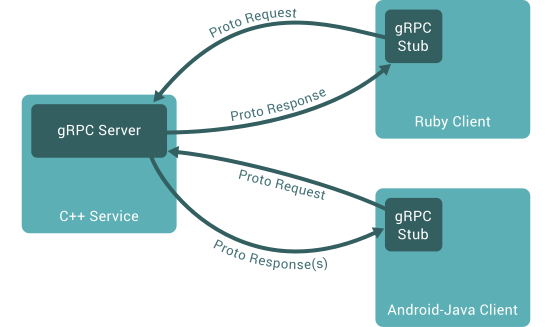
\includegraphics[width=0.8\linewidth]{grpc1.png}
	\caption{Abstract example of different clients using gRPC (Image downloaded from https://grpc.io/docs/what-is-grpc/introduction/ in January 2021)}
	\label{fig:grpcuse}
\end{figure}

As with other RPC frameworks, gRPC allows the client to perform operations as if they were run on the client machine. For this the client needs to be aware of method definition and location of the remote server. To describe these methods gRPC uses protocol buffers \cite{protoBuffer} as the default interface description language (IDL), but it is possible to use other formats (like JSON) through the use of gRPC extensions. The communication with remote server itself is left to the underlying HTTP/2 protocol. 

"Protocol buffers" is a format developed by Google and used to serialize and deserialize structured data, similar to XML. Google describes this format thereby as "think XML, but smaller, faster and simpler" \cite{protoBuffer}. In other words, protocol buffers are a format for structured data, used for the serialization of data and designed to allow the specification of said serialization without a need for additional tooling.

A high-level abstraction of the gRCP intercommunication is shown in figure \ref{fig:grpcuse}. Within this image the gRPC server is written using C++ code. But because of the language agnostic design of gRPC an android phone with a Java client is able to communicate with this server the same way a ruby client is able to.

\begin{lstlisting}[name={Small sample proto buffer specification (Full example available at https://grpc.io/blog/coreos/)},label={code:grpcproto}]  % Start your code-block

service EchoService {
	rpc Echo(EchoMessage) returns (EchoMessage) {
		option (google.api.http) = {
			post: "/v1/echo"
			body: "*"
		};
	}
}
\end{lstlisting}

\begin{figure}
	\centering
	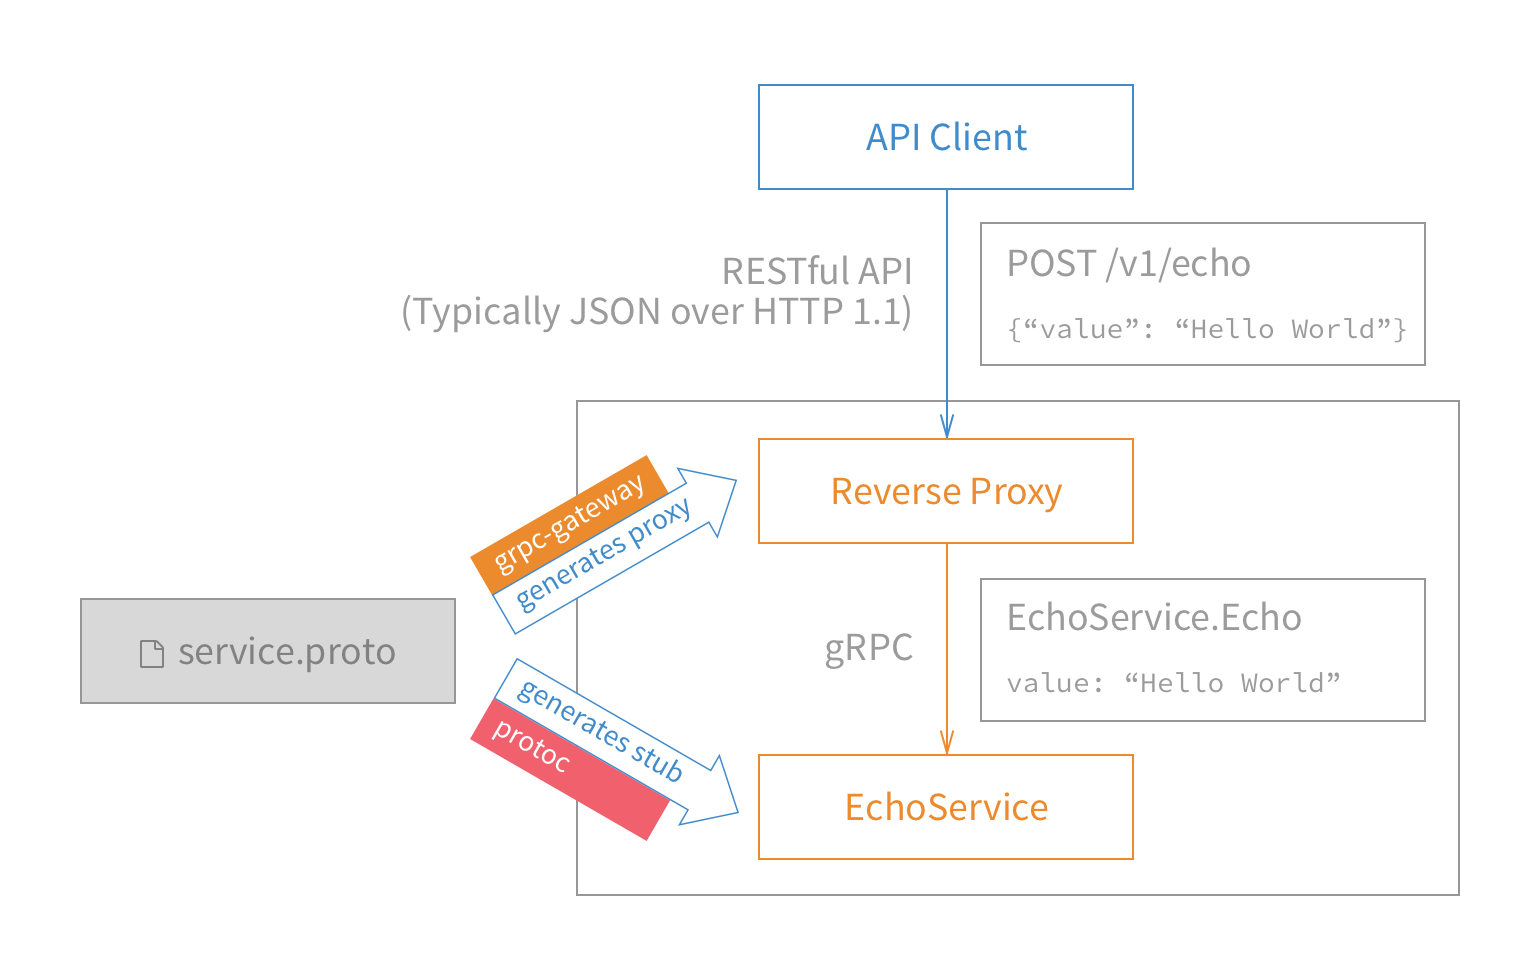
\includegraphics[width=0.8\linewidth]{grpc-rest-gateway.png}
	\caption{Example use of created rest-proxy to communicate with gRPC server (Image downloaded from https://grpc.io/blog/coreos/ in January 2021)}
	\label{fig:restProxy}
\end{figure}

Though gRPC has many advantages in its favor, the framework has the problem that it is requiring the HTTP/2 streaming functionality and the protocol HTTP/2 itself to work. As HTTP/2 is still relatively new not all companies have their infrastructure supporting HTTP/2. As a backwards compatibility to HTTP/1.1 and for general automation support (i.e. no need to import and use stub code) gRPC IDL information can be enhanced with REST options, as shown in listing \ref{code:grpcproto}. These changes will cause the compilation of the IDL to create a rest-proxy in addition to the actual gRPC server. When a client now wants to communicate through REST it may talk with the rest-proxy, which in turn will forward the requests through gRPC to the actual gRCP server. Figure \ref{fig:restProxy} illustrates this communication path and highlights how the created service components are based on the same IDL specification.

As previously mentioned, this makes it possible to have gRPC server and services running within an HTTP/1.1 infrastructure. By HTTP/1.1 infrastructure is hereby meant that not all network components within the infrastructure support the HTTP/2 protocol and have the connections fall back to HTTP/1.1 when trying to communicate through them. Such components could be router, loadbalancer or even the web-server itself. This support makes it possible to introduce new HTTP/2 gRPC services into existing infrastructure and continue using REST with HTTP/1.1 until the network is ready for gRPC. With this any business is able to already start developing gRPC services and start using them to their full potential as soon as their infrastructure becomes ready.

\section{Microservices}
\label{sec:micros}

As the purpose of this paper is to identify the use of REST and gRPC over SOAP in microservice architectures it is necessary to declare the definition that is used for the term microservice. The internet has multiple definition for the term microservice and they may vary on blogs or scientific papers. For the purpose of this document the definition of the national institute of standard and technology (NIST) is used:

"\emph{Microservices: A microservice is a basic element that results from the architectural decomposition of an application’s components into loosely coupled patterns consisting of self-contained services that communicate with each other using a standard communications protocol and a set of well-defined APIs, independent of any vendor, product or technology.}" - NIST \cite{karmel2016nist}

\begin{table}[!htbp]
	\centering
	\caption{Comparison of SOA and Microservices (Karmel, Anil
		Chandramouli, Ramaswamy
		Iorga, Michaela, 2016)}
	\label{micro:comparison}
	\begin{tabular}{| p{0.4\linewidth} | p{0.4\linewidth}|}\hline
		Service Oriented Architecture & Microservice \\\hline
	Self-contained, monolithic services & Small, decomposed, isolated and independently deployable services Communications\\\hline
		Communications between services occur through an enterprise service bus & Communications between services occur through lightweight, standard communications protocols and interfaces\\\hline
		Stateful and requires mapping of service dependencies when changes are introduced & Stateless and less fragile when changes are introduced\\\hline
		Longer start/stop times & Quick start/stop times\\\hline
		Built around services & Built around capabilities\\\hline
	\end{tabular}
\end{table}

Looking at this definition it can be seen that microservice architectures are based on service oriented architectures (SOA) but they drive the decomposition of applications even further. Document "Nist definition of microservices, application containers and system virtual machines" \cite{karmel2016nist} provides us with a comparison between a "standard" SOA and a microservice architecture, as can be seen in table \ref{micro:comparison}. Based on this information, microservices decompose an application not just into services but into capabilities. These "capability services", generally just referred to as services, are to be stateless and allow for independent, fast deployments. In the following section the paper uses the differences outlined in table \ref{micro:comparison} and the definition of the microservice term to analyze the better fitting protocol for a microservice architecture.

\section{Comparison of SOAP and REST for Microservices}
\label{sec:comp}

\begin{table}[!htbp]
	\centering
	\caption{Comparison between SOAP and REST (Wagh \& Thool, 2015)}
	\label{fig:compSoapRest}
	\begin{tabular}{| p{0.4\linewidth} | p{0.4\linewidth}|}\hline
		SOAP & REST \\\hline
		Changing services in SOAP web provisioning often means a complicated code change on the client side. & Changing services in REST web provisioning not requires any change in client side code\\\hline
		SOAP has heavy payload as compared to REST & REST is definitely lightweight as it is meant for lightweight data transfer over a most commonly known interface, - the URI
		It\\\hline
		It requires binary attachment parsing. & It supports all data types directly.\\\hline
		%SOAP is not a wireless infrastructure friendly. & REST is a wireless infrastructure friendly\\\hline
		SOAP web services always return XML data. & While REST web services provide flexibility in regards to the type of data returned.\\\hline
		It consumes more bandwidth because a SOAP response could require more than 10 times as many bytes as compared to REST. & It consumes less bandwidth because it’s response is lightweight.\\\hline
		SOAP request uses POST and require a complex XML request to be created which makes response-caching difficult. & Restful APIs can be consumed using simple GET requests,
		intermediate proxy servers /
		reverse-proxies can cache their response very easily.\\\hline
		SOAP uses HTTP based APIs refer to APIs that are exposed as one or more HTTP URIs and typical responses are in XML / JSON. Response schemas are custom per object & REST on the other hand adds an element of using standrdized URIs, and also giving importance to the HTTP verb used (i.e. GET / POST / PUT etc)\\\hline
		Language, platform, and transport agnostic. & Language and platform agnostic\\\hline
		Designed to handle distributed computing environments. & Assumes a point-to-point communication model; not for distributed computing environment where message may go through one or more intermediaries\\\hline
		Harder to develop, requires tools. & Much simpler to develop web services than SOAP\\\hline
		False assumption: SOAP is more secure. SOAP use WS-Security. WS-Security was created because the SOAP specification was transport-independent and no assumptions could be made about the security available on the transport layer. & REST assumes that the transport will be HTTP (or HTTPS) and the security mechanisms that are built-in to the protocol will be available\\\hline
		%Is the prevailing standard for web services, and hence has better support from other standards (WSDL, WS) and tooling from vendors. & Lack of standards support for security, policy, reliable messaging, etc., so services that have more sophisticated requirements are harder to develop.\\\hline
	\end{tabular}
\end{table}

Sections \ref{sec:soap} and \ref{sec:rest} provide a basic understanding of the SOAP and REST protocol respectively. Together with this knowledge and the comparison of protocols provided by Wagh \& Thool \cite{wagh2012comparative}, shown in table \ref{fig:compSoapRest}, the basis for comparing REST and SOAP on basis of microservices is available.

In addition to the information about the protocols section \ref{sec:micros} provides the definition of microservices. Furthermore the section shows a comparison of requirements between service oriented architectures (SOA) and microservice architectures, as defined in Karmels paper \cite{karmel2016nist}.

When comparing the protocols based on the microservice defintion and requirements of an architecture based on them, it becomes obvious the it is required to use a lightweight communication protocol for interaction between services in said architecture. This lightweight protocol refers both to network traffic and the protocol interface.

Another big requirement of microservice architectures is the ability to use them independently from vendors and technology.

Lastly, the deployments of individual services in a microservice architecture are to be independent from each other and require very loose coupling between the services making up the application.


Because of these reasons this paper focuses on these three categories when analyzing the protocols and there usability for microservice architecture. These categories will be referred to with the following three names in this paper:

\begin{itemize}
	\item Independence
	\item Lightweight Communication Protocol
	\item Deployments
\end{itemize} 

The analysis for each of the categories is found in the following sections, each section containing the information about what protocol better suits the requirements of it.

\subsection{Independence}

NIST requires microservices to use a standard communication protocol and be independent of technologies \cite{karmel2016nist}. If this requirement is applied to SOAP and REST, then table \ref{fig:compSoapRest} identifies one big reason that speaks for the use of REST.

SOAP services always return XML data and do not allow for other formats to be used. REST on the other hand provides a flexibility in the protocol format. It is possible to only support one arbitrary format (like JSON or XML), but it could also be a service that supports multiple formats and the client can decide which of them they require.

Because of this reason the use of REST is better suited for microservice architectures in terms of independence.

\subsection{Lightweight Communication Protocol}

Microservices communicate through lightweight communication protocols and interfaces \cite{karmel2016nist}. On one hand this means that the used protocol should be small in size when transferred through the network and on the other hand this states that the implementation of interfaces should be easy and possible without additional tool requirements.

In terms of payload size the REST protocol is easily the winner in this category. The paper from Wagh \& Thool \cite{wagh2012comparative} emphasizes this point by saying that SOAP has a heavy payload and that REST is definitively lightweight, especially in comparison to SOAP.

The lightweight interface can be argued through the development requirements. SOAP is more complicated and requires tool support, while REST can be implemented with standard tools \cite{wagh2012comparative}. If the development of interfaces is hardly possible without tool support than this speaks against the "lightweight" interface requirement demanded by microservices.

It becomes therefore apparent that in terms of lightweight communication protocols REST is the preferred protocol.

\subsection{Deployments}

In a microservice architecture services need to be loosely coupled and have the ability to be deployed independently from each other \cite{karmel2016nist}. If these services would be built using SOAP as their basis for communication, than this would introduce some coupling and inter-dependence between services. This is the result from having to built classes on the client side that are in line with the WSDL of the services. Not only does this introduce

Generally it is possible to create services based on SOAP and have each of them initially deployed independently, the problem is here on the side of future changes. Wagh \& Thool \cite{wagh2012comparative} identified that changes in SOAP based services may require complicated code changes in clients. Since the microservice definition outright speaks against coupling and dependency, it is easy to understand why REST is preferred over SOAP.

As SOAP introduces tighter coupling between services and reduces the independence of service deployments, REST is better suited for microservice architecture when compared based on the deployment category.  

\section{Comparison of REST and gRPC for Microservices}
\label{sec:compgrpc}

With section \ref{sec:comp} this paper identifies the reasons as to why REST is used instead of SOAP within microservice architectures. This section on the other hand compares the recently emerging gRPC protocol with REST to understand how it can be incorporated into microservice architectures and if it may replace REST in the future. For the general comparison of the protocols this paper takes the categories used in table \ref{fig:compSoapRest} and applies them to gRPC and REST. This means that the protocols will be compared based on:

\begin{itemize}
	\item Coupling between services
	\item Traffic Weight
	\item Protocol Type
	\item Supported Formats
	\item Browser Support
	\item Caching
	\item Complexity of Interface Definition
	\item Technology Dependence
	\item Communication Model
	\item Development Tools and Requirements
	\item Security
\end{itemize}

\begin{table}[!htbp]
	\centering
	\caption{Comparison between REST and gRPC}
	\label{fig:compRestGrpc}
	\begin{tabular}{| p{0.4\linewidth} | p{0.4\linewidth}|}\hline
		REST & gRPC \\\hline
		Changes in REST services do not require changes in clients & Changes in gRPC services require the client to use the newest client stub; Changes are not required if a created REST proxy is used\\\hline
		REST is lightweight and uses the URI and HTTP & gRCP is based on HTTP/2 and uses the URI\\\hline
		Text-based protocol & Binary protocol; REST proxy is text-based.\\\hline
		Supports multiple formats to be used & Supports multiple formats to be used \\\hline
		Restful APIs can be consumed using simple GET requests & Browser do not yet support the capability to directly consume gRPC \\\hline
		Caching of responses with proxies & Supports REST reverse proxy, which can be cached\\\hline
		API defined through standardized URIs and HTTP verbs & API is defined through Interface Definition Language (typically Protocol Buffer); The IDL can be enhanced with REST options to automatically create a REST proxy \\\hline
		Language and platform agnostic & Language and platform agnostic\\\hline
		Assumes a point-to-point communication model; & Point-to-Point Communication\\\hline
		Can be developed using Standard Text-Editors & Can be developed using Standard Text-Editors\\\hline
		Security is provided through use of HTTPS & Security is provided through use of HTTPS\\\hline
	\end{tabular}
\end{table}

Table \ref{fig:compRestGrpc} shows a summary of the answers to these categories (in order of appearance) and can be used as an overview. In the following sections this paper explains the reason behind each of them in detail and follows up with the analysis of gRPCs microservice architecture compatibility.

\subsection{Coupling between services}

Should the services use REST as protocol for interaction, than as shown in table \ref{fig:compSoapRest} and explained in section \ref{sec:rest}, the services do not gain any dependency in their code base. A change within consumed services only causes problems if said alteration introduces a breaking change to existing functionality.

If the services are communicating using gRPC on the other hand, than a change to the service API, outside of breaking changes to existing functionality, may require clients to use the newly generated code stubs. The requirement to use code stubs generated by the server in the client creates a dependency between these services. As gRPC is a framework in addition to a protocol, these generated code stubs are always to be used as libraries in the business code and should therefore not require extensive changes to the overall code base.

\subsection{Traffic Weight}

In terms of traffic usage gRPC is outperforming REST simply through the fact that it is based on the HTTP/2 specification. Corbel, Stephan and Omnes show in their document "HTTP/1.1 pipelining vs HTTP2 in-the-clear: Performance comparison" \cite{7745823} that HTTP/2 is always performing better than HTTP/1.1 when downloading the data for pages.

\subsection{Protocol Type}

REST is a text-based protocol, see \ref{sec:rest}. gRPC on the other hand is binary protocol, see \ref{sec:grpc}.

\subsection{Supported Formats}

The REST protocol supports multiple formats for use (like JSON or XML), see \ref{sec:rest}. gRPC on the other hand is a binary format and only supports multiple IDL specification formats. While the gRPC protocol only supports binary communication, the rest-proxy created through the gRPC framework is able to support multiple non-binary formats (like JSON or XML). Said rest-proxy provides this functionality through the REST protocol and not gRPC.

\subsection{Browser Support}

As REST is using the URI and HTTP for communication it is possible to perform REST requests through the browser, even it some HTTP verbs may require additional plugins for use. In comparison to this gRPC is not supported through browsers, as they would require stub code created by gRPC server to achieve this.

\subsection{Caching}

REST responses can be cached by proxy server \cite{wagh2012comparative}. Responses from a gRPC server on the other hand cannot be cached. Should caching on intermediary proxies be required, a rest-proxy would have to be used.

\subsection{Complexity of Interface Definition}

REST itself uses the URI and HTTP verbs to define the API. It is thereby not required to have a design document, nor is there a fixed standard on how these mechanisms are used to define said API. This makes it possible to directly create a service API within any language, using the languages standard mechanisms.

When creating the gRPC interface on the other hand, an IDL document is to be written that formulates the interaction with the API. While requiring a developer to create an additional file containing the specification, said document can be written using standard text-editors and does not require specialized tools. gRPC achieves this through the use of Protocol Buffers as the default IDL, see section \ref{sec:grpc}.

\subsection{Technology Dependence}

Both protocols support multiple programming languages, see section \ref{sec:rest} and \cite{grpcmotiviation}. Furthermore they can be deployed on any web-server that supports the language used to implement the service.

\subsection{Communication Model}

REST assumes a point-to-point communication model but supports proxies as intermediaries \cite{wagh2012comparative}. gRPC on the other hand requires the client to open a connection directly with server. Use of a rest-proxy makes the actual client use the REST protocol instead of gRPC for communication and does therefore not support gRPC itself with proxy capabilities.

\subsection{Development Tools and Requirements}

As mentioned in subsection \textit{Complexity of Interface Definition}, both protocols interfaces can be created using default text editors. The only tool requirements that may arise are tied to the programming language that is used to implement the API of a service.

\subsection{Security}

Both protocols do not define explicit security mechanisms. Security of transported information is instead provided through use of the HTTPS scheme.

\subsection{Microservices and gRPC}
\label{sec:mgrpc}

gRPC suffers the same problem as SOAP when analyzed for microservice compatibility. The protocol is a RPC framework and requires the client to use the stub created by the gRPC server. Therefore the client now has a dependency on the server service and may require changes when the server is changed. This goes against the loose coupling and independent deployment of microservices \cite{karmel2016nist}.

Additionally, gRPC is a binary protocol and does not fully fit with the independent technology requirement of microservices \cite{karmel2016nist}. While it can be argued that it is possible to use the parsed messages in any programming language and that the IDL can be of different formats, the client is only provided with client code and not with the ability to retrieve the server information in different formats, which would be the actual requirement of microservice architectures.

Based on these points it can be said that gRPC will not replace REST in microservice architectures in the near future. It is still possible to introduce gRPC functionality into certain services of the architecture, but this should only be done if a rest-proxy is additionally provided by the gRPC service. This way the architecture continues to be fully compatible with the microservice definition, but still offer the advantages of streaming requests and responses that gRPC has to the clients that require it.

\section{Conclusion}

This paper provides a comparative analysis of the SOAP, gRPC, and REST styles. For the implementation of microservices, it is essential to choose an appropriate technology to build web services as it influences the implementation and the integration of applications. Lately, REST and gRPC are being chosen over SOAP to implement microservices, and this paper intends to find a suitable explanation. 

REST is a new technique for service abstraction, making the information available under the same rules that command the well-structured microservices. Compared to the SOAP architecture, the RESTful technique presents notable advantages in scalability, coupling, performance, independence of data types, and simplicity in communication, making this the most used technique.

It is noted that gRPC is designed for low latency and high throughput communication. It is excellent for lightweight microservices where efficiency is critical, and it is preferred over SOAP for allowing developers to define any function calls they want, rather than choosing from predefined options and simplifying the otherwise complex remote calls when building APIs for microservices or Docker-based applications, requiring big numbers of remote calls.

Finally, after this research, a more in-depth analysis can be made by comparing the REST and gRPC techniques for microservices. RESTful APIs present advantages over gRPC when it comes to the coupling between services as in REST, no changes are needed, while in gRPC, clients need to update to the newest client stub. Also, REST supports multiple formats to be used, while gRPC only supports binary communication. REST also presents browser support when plugins are needed, while gRPC would require stub code created by the gRPC server to achieve this functionality. Another characteristic is that REST responses can be cached by proxy server while gRPC cannot. REST presents a much simpler interface definition while assuming a point-to-point communication from the client's side while supporting the intermediaries differing from the complex interface definition of gRPC and not supporting intermediaries.

On the other hand, since gRCP is based on HTTP/2, this first is outperforming compared to RESTful APIs since they are implemented on HTTP/1.1. Regarding Development Tools and Requirements, both protocols interfaces can be created using default text editors, and in terms of security, non of the protocols define security mechanisms, and HTTPS is used.

Therefore, although REST and gRCP have made significant steps ahead of SOAP, REST still presents considerably more advantages when it comes to microservices implementations. For the moment, REST cannot be beaten in terms of performance and design, but as times go by and developers experiment with tools, new technologies arise to improve our day to day and interaction with applications.

\bibliography{IEEEabrv,literature}

\end{document}
